\documentclass{article}

\usepackage{fancyhdr}
\usepackage{extramarks}
\usepackage{amsmath}
\usepackage{amsthm}
\usepackage{amsfonts}
\usepackage{tikz}
\usepackage[plain]{algorithm}
%\usepackage{algpseudocode}
\usepackage{amssymb}
\usepackage{enumitem}
\usepackage{relsize}
\usepackage{textcomp}
\usepackage{graphicx}
\usepackage{bm}
\usepackage{wasysym}
%\usepackage{textcomp}
%\usepackage{tabularx}
\usepackage{xcolor,colortbl}

%\usetikzlibrary{automata,positioning}
%\usepgfplotslibrary{external} 
%\tikzexternalize

%
% Basic Document Settings
%

\topmargin=-0.45in
\evensidemargin=0in
\oddsidemargin=0in
\textwidth=6.5in
\textheight=9.0in
\headsep=0.25in

\linespread{1.1}

\pagestyle{fancy}
\lhead{\hmwkAuthorName}
\chead{\hmwkClass\ (\hmwkClassInstructor\ \hmwkClassTime): \hmwkTitle}
\rhead{\hmwkDueDate}
\lfoot{\lastxmark}
\cfoot{\thepage}

\newcommand{\minus}{\scalebox{0.5}[1.0]{$-$}}
\newcommand\tab[1][0.5cm]{\hspace*{#1}}
\renewcommand\headrulewidth{0.4pt}
\renewcommand\footrulewidth{0.4pt}
\renewcommand{\theenumi}{\Alph{enumi}}

\setlength\parindent{0pt}

%
% Create Problem Sections
%

\newcommand{\enterProblemHeader}[1]{
	\nobreak\extramarks{}{{#1} continued on next page\ldots}\nobreak{}
	\nobreak\extramarks{{#1} (continued)}{{#1} continued on next page\ldots}\nobreak{}
}

\newcommand{\exitProblemHeader}[1]{
	\nobreak\extramarks{{#1} (continued)}{{#1} continued on next page\ldots}\nobreak{}
	\stepcounter{homeworkProblemCounter}
	\nobreak\extramarks{{#1}}{}\nobreak{}
}

\newcounter{homeworkProblemCounter}
\setcounter{secnumdepth}{0}
\newcounter{partCounter}
\nobreak\extramarks{Problem \arabic{homeworkProblemCounter}}{}\nobreak{}

\newenvironment{homeworkProblem}[1][-1]{
	\subsection*{{#1}:}
	\enterProblemHeader{{#1}}
	\exitProblemHeader{{#1}}
}

\newcommand{\hmwkTitle}{Homework 6}
\newcommand{\hmwkDueDate}{December 4, 2019}
\newcommand{\hmwkClass}{MTH 5051}
\newcommand{\hmwkClassTime}{Section 01}
\newcommand{\hmwkClassInstructor}{Dr. Jim Jones}
\newcommand{\hmwkAuthorName}{\textbf{Eric Pereira}}

%
% Title Page
%
\pagenumbering{gobble}
\title{
	\vspace{2in}
	\textmd{\textbf{\hmwkClass:\ \hmwkTitle}}\\
	\normalsize\vspace{0.1in}\small{Due\ on\ \hmwkDueDate\ at 11:59pm}\\
	\vspace{0.1in}\large{\textit{\hmwkClassInstructor\ \hmwkClassTime}}
	\vspace{3in}
}

\author{\hmwkAuthorName}
\date{}

\renewcommand{\part}[1]{\textbf{\large Part \Alph{partCounter}}\stepcounter{partCounter}\\}

%
% Various Helper Commands
%

% Useful for algorithms
\newcommand{\alg}[1]{\textsc{\bfseries \footnotesize #1}}

% For derivatives
\newcommand{\deriv}[1]{\frac{\mathrm{d}}{\mathrm{d}x} (#1)}

% For partial derivatives
\newcommand{\pderiv}[2]{\frac{\partial}{\partial #1} (#2)}

% Integral dx
\newcommand{\dx}{\mathrm{d}x}

% Alias for the Solution section header
\newcommand{\solution}{\textbf{\large Solution}}

% Probability commands: Expectation, Variance, Covariance, Bias
\newcommand{\E}{\mathrm{E}}
\newcommand{\Var}{\mathrm{Var}}
\newcommand{\Cov}{\mathrm{Cov}}
\newcommand{\Bias}{\mathrm{Bias}}

\begin{document}
	\maketitle
	
	\pagebreak
	\pagenumbering{arabic}
	
	
	%%%%%%%%%%%%%%%%%%%      
	%	NEW SECTION   %
	%%%%%%%%%%%%%%%%%%%
	\section{Chapter 12.1}
	
	%%%%%%%%%%%%%%%%%%%%%%%%%%%%%%%%%%%%%%%%%%%%%%%%%%%%%%%%%%%%%%%%%%%%%%%%%%%%%%%%%%
	%                                                                                %
	%                          Section 12.1 Problem 1                                %
	%                                                                                %
	%%%%%%%%%%%%%%%%%%%%%%%%%%%%%%%%%%%%%%%%%%%%%%%%%%%%%%%%%%%%%%%%%%%%%%%%%%%%%%%%%%
	
	\begin{homeworkProblem}[Problem 1]
		
		\begin{enumerate}[label=(\alph*)]
			\item Draw the graphs of all nonisomorphic trees on six vertices
			\item How many Isomers does Hexane(C$_6$H$_{14}$) have.
		\end{enumerate}
		
		\textbf{\\Solution:}
		
		\begin{enumerate}[label=(\alph*)]
			\item The trees would look like:
				\begin{center}
					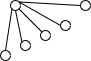
\includegraphics[scale=.6]{photos/12-1-a-PIC1.png}
					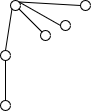
\includegraphics[scale=.6]{photos/12-1-a-PIC2.png}
					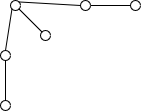
\includegraphics[scale=.6]{photos/12-1-a-PIC3.png}
					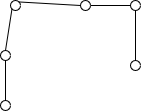
\includegraphics[scale=.6]{photos/12-1-a-PIC4.png}
					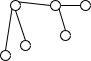
\includegraphics[scale=.6]{photos/12-1-a-PIC5.png}
					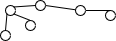
\includegraphics[scale=.6]{photos/12-1-a-PIC6.png}
				\end{center}
			\item There would be a total of 5 isomers. 
		\end{enumerate}
		
	\end{homeworkProblem} 

	%%%%%%%%%%%%%%%%%%%%%%%%%%%%%%%%%%%%%%%%%%%%%%%%%%%%%%%%%%%%%%%%%%%%%%%%%%%%%%%%%%
	%                                                                                %
	%                          Section 12.1 Problem 7                                %
	%                                                                                %
	%%%%%%%%%%%%%%%%%%%%%%%%%%%%%%%%%%%%%%%%%%%%%%%%%%%%%%%%%%%%%%%%%%%%%%%%%%%%%%%%%%
	
	\begin{homeworkProblem}[Problem 7]
		
		\tab Give an example of an undirected graph $G=(V,E)$ where $|V|=|E|+1$ but $G$ is not a tree.
		
		\textbf{\\Solution:\\}
		
		\tab The easy way to create an undirected graph that completes this is to create a small cycle, and a vertice on the outside of the connected graph. This would look like:
		\begin{center}
			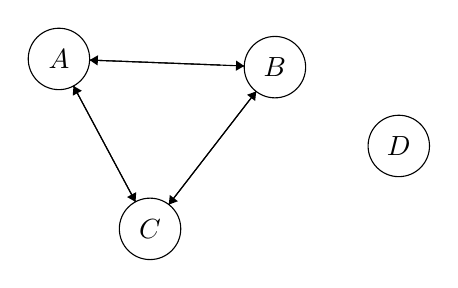
\begin{tikzpicture}[scale=0.13]
			\tikzstyle{every node}+=[inner sep=0pt]
			\draw [black] (17.1,-12.5) circle (3);
			\draw (17.1,-12.5) node {$A$};
			\draw [black] (38.2,-13.3) circle (3);
			\draw (38.2,-13.3) node {$B$};
			\draw [black] (26,-29.1) circle (3);
			\draw (26,-29.1) node {$C$};
			\draw [black] (50.3,-21) circle (3);
			\draw (50.3,-21) node {$D$};
			\draw [black] (18.52,-15.14) -- (24.58,-26.46);
			\fill [black] (24.58,-26.46) -- (24.65,-25.51) -- (23.76,-25.99);
			\draw [black] (24.58,-26.46) -- (18.52,-15.14);
			\fill [black] (18.52,-15.14) -- (18.45,-16.09) -- (19.34,-15.61);
			\draw [black] (32.9,-13.1) -- (20.1,-12.61);
			\fill [black] (20.1,-12.61) -- (20.88,-13.14) -- (20.92,-12.14);
			\draw [black] (20.1,-12.61) -- (35.2,-13.19);
			\fill [black] (35.2,-13.19) -- (34.42,-12.66) -- (34.38,-13.66);
			\draw [black] (36.37,-15.67) -- (27.83,-26.73);
			\fill [black] (27.83,-26.73) -- (28.72,-26.4) -- (27.93,-25.79);
			\draw [black] (27.83,-26.73) -- (36.37,-15.67);
			\fill [black] (36.37,-15.67) -- (35.48,-16) -- (36.27,-16.61);
			\end{tikzpicture}
		\end{center}
		
	\end{homeworkProblem} 

	%%%%%%%%%%%%%%%%%%%%%%%%%%%%%%%%%%%%%%%%%%%%%%%%%%%%%%%%%%%%%%%%%%%%%%%%%%%%%%%%%%
	%                                                                                %
	%                          Section 12.1 Problem 9                                %
	%                                                                                %
	%%%%%%%%%%%%%%%%%%%%%%%%%%%%%%%%%%%%%%%%%%%%%%%%%%%%%%%%%%%%%%%%%%%%%%%%%%%%%%%%%%
	
	\begin{homeworkProblem}[Problem 9]
		
		\tab If $G=(V,E)$ is a loop-free undirected graph, prove that $G$ is a tree if there is a unique path between any two vertices of $G$.
		
		\textbf{\\Solution:\\}
		
		
	\end{homeworkProblem} 

	%%%%%%%%%%%%%%%%%%%      
	%	NEW SECTION   %
	%%%%%%%%%%%%%%%%%%%
	\section{Chapter 12.2}
	
	%%%%%%%%%%%%%%%%%%%%%%%%%%%%%%%%%%%%%%%%%%%%%%%%%%%%%%%%%%%%%%%%%%%%%%%%%%%%%%%%%%
	%                                                                                %
	%                          Section 12.2 Problem 5                                %
	%                                                                                %
	%%%%%%%%%%%%%%%%%%%%%%%%%%%%%%%%%%%%%%%%%%%%%%%%%%%%%%%%%%%%%%%%%%%%%%%%%%%%%%%%%%
	
	\begin{homeworkProblem}[Problem 5]
		\tab For the tree shown in Fig. 12.30, list the vertices according to a preorder traversal, an inorder traversal, and a postorder traversal.
		
		\begin{center}
			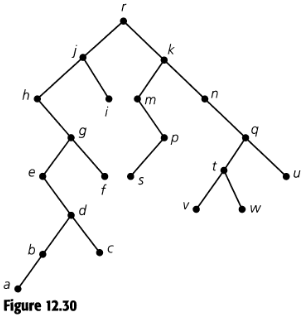
\includegraphics[scale=.7]{photos/FIG1230.png}
		\end{center}
		
		\textbf{\\Solution:\\}
		
		\tab The different traversals would look like this:
		\begin{align*}
			&\text{preorder:}  &\text{r,j,h,g,e,d,b,a,c,f,i,k,m,p,s,n,q,t,v,w,u} \\
			&\text{inorder:} &\text{h,e,a,b,d,c,g,f,j,i,r,m,s,p,k,n,v,t,w,q,u} \\
			&\text{postorder:} &\text{a,b,c,d,e,f,g,h,i,j,s,p,m,v,w,t,u,q,n,k,r}
		\end{align*}
	\end{homeworkProblem} 

	%%%%%%%%%%%%%%%%%%%%%%%%%%%%%%%%%%%%%%%%%%%%%%%%%%%%%%%%%%%%%%%%%%%%%%%%%%%%%%%%%%
	%                                                                                %
	%                          Section 12.2 Problem 7a                               %
	%                                                                                %
	%%%%%%%%%%%%%%%%%%%%%%%%%%%%%%%%%%%%%%%%%%%%%%%%%%%%%%%%%%%%%%%%%%%%%%%%%%%%%%%%%%
	
	\begin{homeworkProblem}[Problem 7a]
		
		\tab Find the depth-first spanning tree for the graph shown in Fig. 11.72(a) if the order of the vertices is given as 
		\begin{enumerate}[label=(\roman*)]
			\item a,b,c,d,e,f,g,h;
			\item h,g,f,e,d,c,b,a;
			\item a,b,c,d,h,g,f,e;
		\end{enumerate}
		\begin{center}
			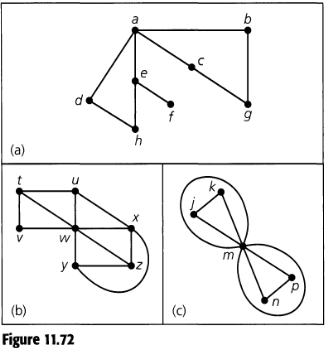
\includegraphics[scale=.7]{photos/FIG1172.png}
		\end{center}
		
		\textbf{\\Solution:}
		\begin{enumerate}[label=(\roman*)]
			\item For this patter, if you traverse (a) it would end up looking like:
				\begin{center}
					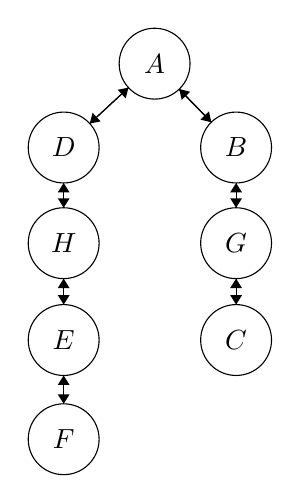
\begin{tikzpicture}[scale=0.15]
					\tikzstyle{every node}+=[inner sep=0pt]
					\draw [black] (37.5,-11.7) circle (3);
					\draw (37.5,-11.7) node {$A$};
					\draw [black] (29.8,-18.8) circle (3);
					\draw (29.8,-18.8) node {$D$};
					\draw [black] (44.4,-18.8) circle (3);
					\draw (44.4,-18.8) node {$B$};
					\draw [black] (44.4,-26.9) circle (3);
					\draw (44.4,-26.9) node {$G$};
					\draw [black] (29.8,-26.9) circle (3);
					\draw (29.8,-26.9) node {$H$};
					\draw [black] (29.8,-35.1) circle (3);
					\draw (29.8,-35.1) node {$E$};
					\draw [black] (44.4,-35.1) circle (3);
					\draw (44.4,-35.1) node {$C$};
					\draw [black] (29.8,-43.5) circle (3);
					\draw (29.8,-43.5) node {$F$};
					\draw [black] (39.6,-13.9) -- (42.3,-16.66);
					\fill [black] (42.3,-16.66) -- (42.1,-15.74) -- (41.38,-16.44);
					\draw [black] (42.31,-16.65) -- (39.59,-13.85);
					\fill [black] (39.59,-13.85) -- (39.79,-14.77) -- (40.51,-14.08);
					\draw [black] (35.29,-13.73) -- (32.01,-16.77);
					\fill [black] (32.01,-16.77) -- (32.93,-16.59) -- (32.25,-15.86);
					\draw [black] (32.01,-16.77) -- (35.29,-13.73);
					\fill [black] (35.29,-13.73) -- (34.37,-13.91) -- (35.05,-14.64);
					\draw [black] (29.8,-21.8) -- (29.8,-23.9);
					\fill [black] (29.8,-23.9) -- (30.3,-23.1) -- (29.3,-23.1);
					\draw [black] (29.8,-23.9) -- (29.8,-21.8);
					\fill [black] (29.8,-21.8) -- (29.3,-22.6) -- (30.3,-22.6);
					\draw [black] (29.8,-30) -- (29.8,-32.1);
					\fill [black] (29.8,-32.1) -- (30.3,-31.3) -- (29.3,-31.3);
					\draw [black] (29.8,-32.1) -- (29.8,-29.9);
					\fill [black] (29.8,-29.9) -- (29.3,-30.7) -- (30.3,-30.7);
					\draw [black] (29.8,-38.1) -- (29.8,-40.5);
					\fill [black] (29.8,-40.5) -- (30.3,-39.7) -- (29.3,-39.7);
					\draw [black] (29.8,-40.5) -- (29.8,-38.1);
					\fill [black] (29.8,-38.1) -- (29.3,-38.9) -- (30.3,-38.9);
					\draw [black] (44.4,-21.9) -- (44.4,-23.9);
					\fill [black] (44.4,-23.9) -- (44.9,-23.1) -- (43.9,-23.1);
					\draw [black] (44.4,-23.9) -- (44.4,-21.8);
					\fill [black] (44.4,-21.8) -- (43.9,-22.6) -- (44.9,-22.6);
					\draw [black] (44.4,-29.9) -- (44.4,-32.1);
					\fill [black] (44.4,-32.1) -- (44.9,-31.3) -- (43.9,-31.3);
					\draw [black] (44.4,-32.1) -- (44.4,-29.9);
					\fill [black] (44.4,-29.9) -- (43.9,-30.7) -- (44.9,-30.7);
					\end{tikzpicture}
				\end{center}
			\item if you instead go backwards it would end up looking like:
				\begin{center}
					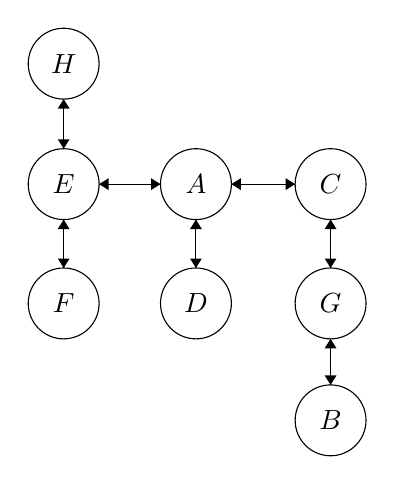
\begin{tikzpicture}[scale=0.15]
					\tikzstyle{every node}+=[inner sep=0pt]
					\draw [black] (31,-11.2) circle (3);
					\draw (31,-11.2) node {$H$};
					\draw [black] (31,-21.4) circle (3);
					\draw (31,-21.4) node {$E$};
					\draw [black] (31,-31.5) circle (3);
					\draw (31,-31.5) node {$F$};
					\draw [black] (42.2,-21.4) circle (3);
					\draw (42.2,-21.4) node {$A$};
					\draw [black] (42.2,-31.5) circle (3);
					\draw (42.2,-31.5) node {$D$};
					\draw [black] (53.6,-21.4) circle (3);
					\draw (53.6,-21.4) node {$C$};
					\draw [black] (53.6,-31.5) circle (3);
					\draw (53.6,-31.5) node {$G$};
					\draw [black] (53.6,-41.4) circle (3);
					\draw (53.6,-41.4) node {$B$};
					\draw [black] (31,-14.2) -- (31,-18.4);
					\fill [black] (31,-18.4) -- (31.5,-17.6) -- (30.5,-17.6);
					\draw [black] (31,-18.4) -- (31,-14.2);
					\fill [black] (31,-14.2) -- (30.5,-15) -- (31.5,-15);
					\draw [black] (31,-24.4) -- (31,-28.5);
					\fill [black] (31,-28.5) -- (31.5,-27.7) -- (30.5,-27.7);
					\draw [black] (31,-28.5) -- (31,-24.4);
					\fill [black] (31,-24.4) -- (30.5,-25.2) -- (31.5,-25.2);
					\draw [black] (45.2,-21.4) -- (50.6,-21.4);
					\fill [black] (50.6,-21.4) -- (49.8,-20.9) -- (49.8,-21.9);
					\draw [black] (42.2,-24.4) -- (42.2,-28.5);
					\fill [black] (42.2,-28.5) -- (42.7,-27.7) -- (41.7,-27.7);
					\draw [black] (42.2,-28.5) -- (42.2,-24.4);
					\fill [black] (42.2,-24.4) -- (41.7,-25.2) -- (42.7,-25.2);
					\draw [black] (50.6,-21.4) -- (45.2,-21.4);
					\fill [black] (45.2,-21.4) -- (46,-21.9) -- (46,-20.9);
					\draw [black] (53.6,-24.4) -- (53.6,-28.5);
					\fill [black] (53.6,-28.5) -- (54.1,-27.7) -- (53.1,-27.7);
					\draw [black] (53.6,-28.5) -- (53.6,-24.4);
					\fill [black] (53.6,-24.4) -- (53.1,-25.2) -- (54.1,-25.2);
					\draw [black] (35,-21.4) -- (39.2,-21.4);
					\fill [black] (39.2,-21.4) -- (38.4,-20.9) -- (38.4,-21.9);
					\draw [black] (39.2,-21.4) -- (34,-21.4);
					\fill [black] (34,-21.4) -- (34.8,-21.9) -- (34.8,-20.9);
					\draw [black] (53.6,-34.5) -- (53.6,-38.4);
					\fill [black] (53.6,-38.4) -- (54.1,-37.6) -- (53.1,-37.6);
					\draw [black] (53.6,-38.4) -- (53.6,-34.5);
					\fill [black] (53.6,-34.5) -- (53.1,-35.3) -- (54.1,-35.3);
					\end{tikzpicture}
				\end{center}
			\item This actually ends being exactly the same as (i) spanning tree and would look like:
				\begin{center}
					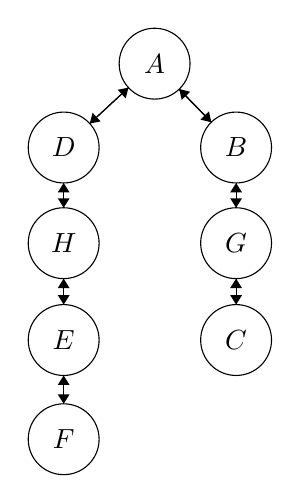
\begin{tikzpicture}[scale=0.15]
					\tikzstyle{every node}+=[inner sep=0pt]
					\draw [black] (37.5,-11.7) circle (3);
					\draw (37.5,-11.7) node {$A$};
					\draw [black] (29.8,-18.8) circle (3);
					\draw (29.8,-18.8) node {$D$};
					\draw [black] (44.4,-18.8) circle (3);
					\draw (44.4,-18.8) node {$B$};
					\draw [black] (44.4,-26.9) circle (3);
					\draw (44.4,-26.9) node {$G$};
					\draw [black] (29.8,-26.9) circle (3);
					\draw (29.8,-26.9) node {$H$};
					\draw [black] (29.8,-35.1) circle (3);
					\draw (29.8,-35.1) node {$E$};
					\draw [black] (44.4,-35.1) circle (3);
					\draw (44.4,-35.1) node {$C$};
					\draw [black] (29.8,-43.5) circle (3);
					\draw (29.8,-43.5) node {$F$};
					\draw [black] (39.6,-13.9) -- (42.3,-16.66);
					\fill [black] (42.3,-16.66) -- (42.1,-15.74) -- (41.38,-16.44);
					\draw [black] (42.31,-16.65) -- (39.59,-13.85);
					\fill [black] (39.59,-13.85) -- (39.79,-14.77) -- (40.51,-14.08);
					\draw [black] (35.29,-13.73) -- (32.01,-16.77);
					\fill [black] (32.01,-16.77) -- (32.93,-16.59) -- (32.25,-15.86);
					\draw [black] (32.01,-16.77) -- (35.29,-13.73);
					\fill [black] (35.29,-13.73) -- (34.37,-13.91) -- (35.05,-14.64);
					\draw [black] (29.8,-21.8) -- (29.8,-23.9);
					\fill [black] (29.8,-23.9) -- (30.3,-23.1) -- (29.3,-23.1);
					\draw [black] (29.8,-23.9) -- (29.8,-21.8);
					\fill [black] (29.8,-21.8) -- (29.3,-22.6) -- (30.3,-22.6);
					\draw [black] (29.8,-30) -- (29.8,-32.1);
					\fill [black] (29.8,-32.1) -- (30.3,-31.3) -- (29.3,-31.3);
					\draw [black] (29.8,-32.1) -- (29.8,-29.9);
					\fill [black] (29.8,-29.9) -- (29.3,-30.7) -- (30.3,-30.7);
					\draw [black] (29.8,-38.1) -- (29.8,-40.5);
					\fill [black] (29.8,-40.5) -- (30.3,-39.7) -- (29.3,-39.7);
					\draw [black] (29.8,-40.5) -- (29.8,-38.1);
					\fill [black] (29.8,-38.1) -- (29.3,-38.9) -- (30.3,-38.9);
					\draw [black] (44.4,-21.9) -- (44.4,-23.9);
					\fill [black] (44.4,-23.9) -- (44.9,-23.1) -- (43.9,-23.1);
					\draw [black] (44.4,-23.9) -- (44.4,-21.8);
					\fill [black] (44.4,-21.8) -- (43.9,-22.6) -- (44.9,-22.6);
					\draw [black] (44.4,-29.9) -- (44.4,-32.1);
					\fill [black] (44.4,-32.1) -- (44.9,-31.3) -- (43.9,-31.3);
					\draw [black] (44.4,-32.1) -- (44.4,-29.9);
					\fill [black] (44.4,-29.9) -- (43.9,-30.7) -- (44.9,-30.7);
					\end{tikzpicture}
				\end{center} 
		\end{enumerate}
		
	\end{homeworkProblem} 

	%%%%%%%%%%%%%%%%%%%%%%%%%%%%%%%%%%%%%%%%%%%%%%%%%%%%%%%%%%%%%%%%%%%%%%%%%%%%%%%%%%
	%                                                                                %
	%                          Section 12.2 Problem 11                               %
	%                                                                                %
	%%%%%%%%%%%%%%%%%%%%%%%%%%%%%%%%%%%%%%%%%%%%%%%%%%%%%%%%%%%%%%%%%%%%%%%%%%%%%%%%%%
	
	\begin{homeworkProblem}[Problem 11]
		\tab Prove Theorom 12.6 and Corollary 12.1. \\
		
		\tab Theorom 12.6: Let $T = (V, E)$ be a complete $m$-ary tree with $|V| = n$. If $T$ has $\ell$ leaves and $i$ internal vertices, then
		\begin{enumerate}[label=(\alph*)]
			\item $n=mi+1$;
			\item $\ell=(m-1)i+1$;
			\item and $i=\dfrac{\ell-1}{m-1}=\dfrac{n-1}{m}$
		\end{enumerate}
	
		Corollary 12.1: Let $T$ be a balanced complete $m$-ary tree with $\ell$ leaves. Then the height of $T$ is [$\log_m\ell$].
		
		\textbf{\\Solution:\\}
		
		
	\end{homeworkProblem} 
	%%%%%%%%%%%%%%%%%%%      
	%	NEW SECTION   %
	%%%%%%%%%%%%%%%%%%%
	\section{Chapter 12.3}
	
	%%%%%%%%%%%%%%%%%%%%%%%%%%%%%%%%%%%%%%%%%%%%%%%%%%%%%%%%%%%%%%%%%%%%%%%%%%%%%%%%%%
	%                                                                                %
	%                          Section 12.3 Problem 1                                %
	%                                                                                %
	%%%%%%%%%%%%%%%%%%%%%%%%%%%%%%%%%%%%%%%%%%%%%%%%%%%%%%%%%%%%%%%%%%%%%%%%%%%%%%%%%%
	
	\begin{homeworkProblem}[Problem 1]
		\begin{enumerate}[label=(\alph*)]
			\item Give an example of two lists $L_1$, $L_2$, each of which is in ascending order and contains five elements, and where nine comparisons are needed to merge $L_1$, $L_2$ by the algorithm given in Lemma 12.1.
			\item Let $m$, $n\in \mathbb{Z}^+$ with $m < n$. Give an example of two lists $L_1$, $L_2$, each of which is in ascending order, where $L_1$ has $m$ elements, $L_2$ has $n$ elements, and $m + n — 1$ comparisons are needed to merge $L_1$, $L_2$ by the algorithm given in Lemma 12.1.
		\end{enumerate}
		
		\textbf{\\Solution:}
		\begin{enumerate}[label=(\alph*)]
			\item 
			\item 
		\end{enumerate}
		
		
	\end{homeworkProblem} 
	
	%%%%%%%%%%%%%%%%%%%%%%%%%%%%%%%%%%%%%%%%%%%%%%%%%%%%%%%%%%%%%%%%%%%%%%%%%%%%%%%%%%
	%                                                                                %
	%                          Section 12.3 Problem 2                                %
	%                                                                                %
	%%%%%%%%%%%%%%%%%%%%%%%%%%%%%%%%%%%%%%%%%%%%%%%%%%%%%%%%%%%%%%%%%%%%%%%%%%%%%%%%%%
	
	\begin{homeworkProblem}[Problem 2]
		\tab Apply the merge sort to each of the following lists. Draw the splitting and merging trees for each application of the procedure.
		
		\begin{enumerate}[label=(\alph*)]
			\item -1, 0, 2, -2, 3, 6, -3, 5, 1,4
			\item -1, 7, 4, 11, 5, -8, 15, -3, -2, 6, 10, 3 
		\end{enumerate}
		
		\textbf{\\Solution:}
		
		\begin{enumerate}[label=(\alph*)]
			\item Initially we need to start dividing each into individual pieces, so we are going to completely separate the the list. This initial separation would look like:
			\begin{center}
				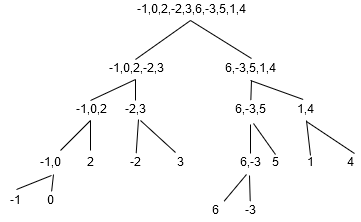
\includegraphics[scale=.58]{photos/12-3-2-a-1.png}
			\end{center}
			\tab Now, it is separated so at this point we would perform the merge where the actual magic happens, this would look like:
			\begin{center}
				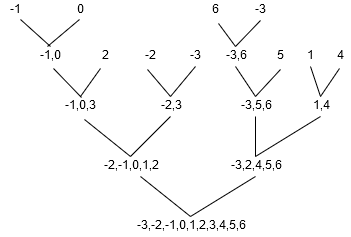
\includegraphics[scale=.58]{photos/12-3-2-a-2.png}
			\end{center}
			\item 
		\end{enumerate}
		
		
	\end{homeworkProblem} 
	
	%%%%%%%%%%%%%%%%%%%%%%%%%%%%%%%%%%%%%%%%%%%%%%%%%%%%%%%%%%%%%%%%%%%%%%%%%%%%%%%%%%
	%                                                                                %
	%                          Section 12.3 Problem 3                                %
	%                                                                                %
	%%%%%%%%%%%%%%%%%%%%%%%%%%%%%%%%%%%%%%%%%%%%%%%%%%%%%%%%%%%%%%%%%%%%%%%%%%%%%%%%%%
	
	\begin{homeworkProblem}[Problem 3]
		\tab Related to the merge sort is a somewhat more efficient procedure called the quick sort. Here we start with a list
		$L: a_1, a_2, ..., a_n$, and use $a_1$ as a pivot to develop two sublists $L_1$ and $L_2$ as follows. For $i > 1$, if $a_i < a_1$, place $a_i$ at the end of the first list being developed (this is $L_1$ at the end of the process); otherwise, place a, at the end of the second list $L_2$.
		
		\tab After all $a_1$, $i > 1$, have been processed, place $a_1$ at the end of the first list. Now apply quick sort recursively to each of the lists $L_1$ and $L_2$ to obtain sublists $L_{11}$, $L_{12}$, $L_{21}$, and $L_{22}$. Continue the process until each of the resulting sublists contains one element. The sublists are then ordered, and their concatenation gives the ordering sought for the original list $L$.
		
		\tab Apply quick sort to each list in Exercise 2.
		
		\textbf{\\Solution:}
		
		\begin{enumerate}[label=(\alph*)]
			\item 
			\item 
		\end{enumerate}
		
	\end{homeworkProblem} 

	%%%%%%%%%%%%%%%%%%%      
	%	NEW SECTION   %
	%%%%%%%%%%%%%%%%%%%
	\section{Chapter 12.4}
	
	%%%%%%%%%%%%%%%%%%%%%%%%%%%%%%%%%%%%%%%%%%%%%%%%%%%%%%%%%%%%%%%%%%%%%%%%%%%%%%%%%%
	%                                                                                %
	%                          Section 12.4 Problem 3                                %
	%                                                                                %
	%%%%%%%%%%%%%%%%%%%%%%%%%%%%%%%%%%%%%%%%%%%%%%%%%%%%%%%%%%%%%%%%%%%%%%%%%%%%%%%%%%
	
	\begin{homeworkProblem}[Problem 3]
		\tab Construct an optimal prefix code for the symbols $a, b, c, ..., i, j$ that occur (in a given sample) with respective frequencies 78, 16, 30, 35, 125, 31, 20, 50, 80, 3.
		
		\textbf{\\Solution:}
		
		
	\end{homeworkProblem} 

	%%%%%%%%%%%%%%%%%%%      
	%	NEW SECTION   %
	%%%%%%%%%%%%%%%%%%%
	\section{Chapter 12.5}
	
	%%%%%%%%%%%%%%%%%%%%%%%%%%%%%%%%%%%%%%%%%%%%%%%%%%%%%%%%%%%%%%%%%%%%%%%%%%%%%%%%%%
	%                                                                                %
	%                          Section 12.5 Problem 1                                %
	%                                                                                %
	%%%%%%%%%%%%%%%%%%%%%%%%%%%%%%%%%%%%%%%%%%%%%%%%%%%%%%%%%%%%%%%%%%%%%%%%%%%%%%%%%%
	
	\begin{homeworkProblem}[Problem 1]
		\tab Find the articulation points and biconnected components for the graph shown in Fig. 12.44
		\begin{center}
			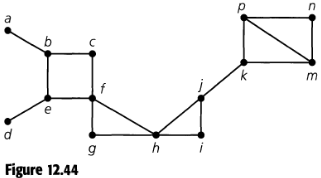
\includegraphics[scale=1]{photos/FIG1244.png}
		\end{center}
		
		\textbf{\\Solution:\\}
		
		
	\end{homeworkProblem} 
	
	%%%%%%%%%%%%%%%%%%%%%%%%%%%%%%%%%%%%%%%%%%%%%%%%%%%%%%%%%%%%%%%%%%%%%%%%%%%%%%%%%%
	%                                                                                %
	%                          Section 12.5 Problem 3                                %
	%                                                                                %
	%%%%%%%%%%%%%%%%%%%%%%%%%%%%%%%%%%%%%%%%%%%%%%%%%%%%%%%%%%%%%%%%%%%%%%%%%%%%%%%%%%
	
	\begin{homeworkProblem}[Problem 3]
		\tab Let $T = (V, E)$ be a tree with $|V| = n > 3$.
		\begin{enumerate}[label=(\alph*)]
			\item What are the smallest and the largest numbers of articulation points that $T$ can have? Describe the trees for each of these cases.
			\item How many biconnected components does $T$ have in each of the cases in part (a)?
		\end{enumerate}
		
		\textbf{\\Solution:}
		
		
	\end{homeworkProblem} 
	
	%%%%%%%%%%%%%%%%%%%%%%%%%%%%%%%%%%%%%%%%%%%%%%%%%%%%%%%%%%%%%%%%%%%%%%%%%%%%%%%%%%
	%                                                                                %
	%                          Section 12.5 Problem 7                                %
	%                                                                                %
	%%%%%%%%%%%%%%%%%%%%%%%%%%%%%%%%%%%%%%%%%%%%%%%%%%%%%%%%%%%%%%%%%%%%%%%%%%%%%%%%%%
	
	\begin{homeworkProblem}[Problem 7]
		\tab Let $G = (V, E)$ be a loop-free connected undirected graph with $|V| > 3$. If $G$ has no articulation points, prove that $G$ has no pendant vertices.
		
		\textbf{\\Solution:}
		
		
	\end{homeworkProblem}

	%%%%%%%%%%%%%%%%%%%%%%%%%%%%%%%%%%%%%%%%%%%%%%%%%%%%%%%%%%%%%%%%%%%%%%%%%%%%%%%%%%
	%                                                                                %
	%                          Section 12.5 Problem 9                                %
	%                                                                                %
	%%%%%%%%%%%%%%%%%%%%%%%%%%%%%%%%%%%%%%%%%%%%%%%%%%%%%%%%%%%%%%%%%%%%%%%%%%%%%%%%%%
	
	\begin{homeworkProblem}[Problem 9]
		\tab Answer the questions posed in the previous exercise but this time order the vertices as $h, g, f, e, d, c, b, a$ and let $c$ be the root of $T$.
		\begin{center}
			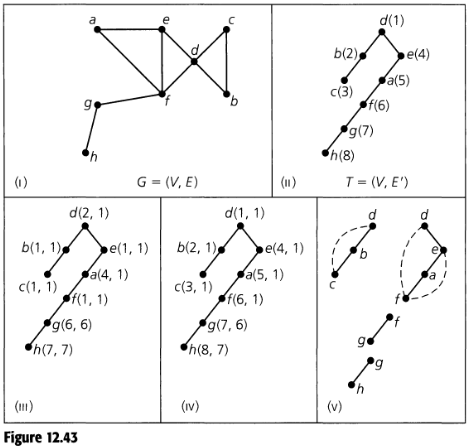
\includegraphics[scale=.7]{photos/FIG1243.png}
		\end{center}
		
		\textbf{\\Solution:\\}
		
		
	\end{homeworkProblem}

	%%%%%%%%%%%%%%%%%%%      
	%	NEW SECTION   %
	%%%%%%%%%%%%%%%%%%%
	\section{Chapter 13.2}
	
	%%%%%%%%%%%%%%%%%%%%%%%%%%%%%%%%%%%%%%%%%%%%%%%%%%%%%%%%%%%%%%%%%%%%%%%%%%%%%%%%%%
	%                                                                                %
	%                          Section 13.2 Problem 3                                %
	%                                                                                %
	%%%%%%%%%%%%%%%%%%%%%%%%%%%%%%%%%%%%%%%%%%%%%%%%%%%%%%%%%%%%%%%%%%%%%%%%%%%%%%%%%%
	
	\begin{homeworkProblem}[Problem 3]
		\tab Let $G = (V, E)$ be a loop-free weighted connected undirected graph with $T =(V, E)$,a minimal spanning tree for $G$. For $v, w \in V$, is the path from $v$ to $w$ in $T$ a path of minimum weight in $G$?
		
		\textbf{\\Solution:}
		
		
	\end{homeworkProblem} 
	
	%%%%%%%%%%%%%%%%%%%%%%%%%%%%%%%%%%%%%%%%%%%%%%%%%%%%%%%%%%%%%%%%%%%%%%%%%%%%%%%%%%
	%                                                                                %
	%                          Section 13.2 Problem 4                                %
	%                                                                                %
	%%%%%%%%%%%%%%%%%%%%%%%%%%%%%%%%%%%%%%%%%%%%%%%%%%%%%%%%%%%%%%%%%%%%%%%%%%%%%%%%%%
	
	\begin{homeworkProblem}[Problem 4]
		\tab Table 13.1 provides information on the distance (in miles) between pairs of cities in the state of Indiana.
		
		\tab A system of highways connecting these seven cities is to be constructed. Determine which highways should be constructed to that the cost of construction is minimal. (Assume that the cost of construction of a mile of highway is the same between every pair of cities.) 		
		
		\begin{center}
			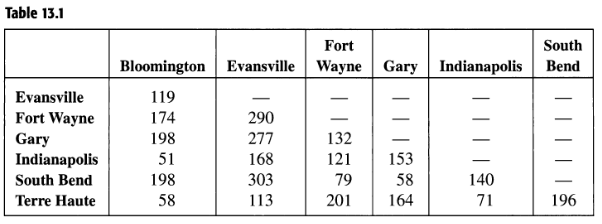
\includegraphics[scale=.7]{photos/TAB131.png}
		\end{center}
		
		\textbf{\\Solution:\\}
		
		\tab Primarily, it is important to understand the main focus. This can be done by connecting the cities: \\
		
		\begin{center}
			Gary - South Bend (58 miles), South Bend - Fort Wayne (79 miles), \\ Fort Wayne - Indianapolis (121 miles), Indianapolis - Bloomington (51 miles), \\ Bloomington - Terre Haute (58 Miles), Terre Haute - Evansville (113 miles)
		\end{center}
	
		\tab This would result in a total of 480 miles of road. 
		
		
		
	\end{homeworkProblem} 
	
	%%%%%%%%%%%%%%%%%%%%%%%%%%%%%%%%%%%%%%%%%%%%%%%%%%%%%%%%%%%%%%%%%%%%%%%%%%%%%%%%%%
	%                                                                                %
	%                          Section 13.2 Problem 9                                %
	%                                                                                %
	%%%%%%%%%%%%%%%%%%%%%%%%%%%%%%%%%%%%%%%%%%%%%%%%%%%%%%%%%%%%%%%%%%%%%%%%%%%%%%%%%%
	
	\begin{homeworkProblem}[Problem 9]
		\tab Let $G = (V, E)$ be a loop-free weighted connected undirected graph, where for each pair of distinct edges $e_1, e_2 \in E$, $wt(e_1) \ne wt(e_2)$. Prove that $G$ has only one minimal spanning tree.
		
		\textbf{\\Solution:\\}
		
		\tab According to Kruskals algorithm earlier in the chapter, there are distinct
		
	\end{homeworkProblem}

\end{document}